\documentclass[12pt, a4paper]{article}
\usepackage{bm, float,amsmath,graphicx}
\graphicspath{ {./images/} }
\usepackage[T1]{fontenc}
\usepackage[polish]{babel}
\usepackage[utf8]{inputenc}

\title{Opracowanie zadania z geometrii obliczeniowej}
\author{Stepan Yurtsiv, 246437}

\begin{document}
\maketitle

\section*{Zadanie}

Niech $S'$ będzie zbiorem środków okręgów jednostkowych ze zbioru $S$. Pokaż, że okrąg z $S$ pojawia się na brzegu otoczki wypukłej wtedy i tylko wtedy, gdy jego środek
leży na brzegu otoczki wypukłej $S'$. Podaj algorytm obliczania otoczki wypukłej $S$ pracujący w czasie $O(n\log n)$ (zadanie 26 na liście).


\section*{Rozwiązanie}

\subsection*{Część pierwsza}

Na rysunku \ref{fig:img1} na pomarańczowo jest narysowana otoczka wypukła $S'$ oraz na zielono otoczka $S$. 
Widać że punkt wewnątrz otoczki $S'$ musiałby leżeć na którymś z odcinków otoczki $S'$ żeby odpowiedni okrąg był
częszcią $S$ lub ten okrąg musiałby mieć większy promień od innych okręgów.

\begin{figure}[H]
  \begin{center}
  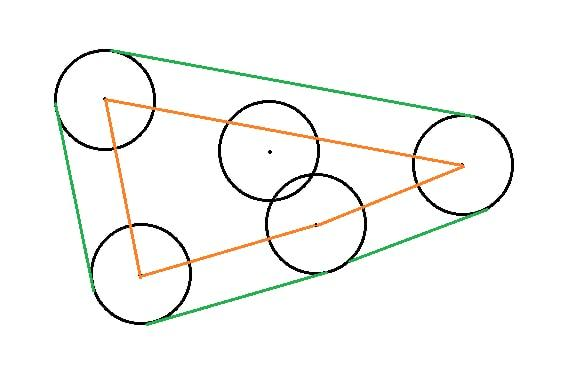
\includegraphics[scale=0.65]{Img1}
  \caption{$S$ i $S'$}
  \label{fig:img1}
  \end{center}
\end{figure}

\subsection*{Algorytm}

Żeby znaleźć otoczkę wypukłą $S$, wystarczy najpierw stworzyć otoczkę wypukłą $S'$ dla zbioru
środków okręgów, następnie z każdego punktu otoczki $S'$ poprowadzić proste prostopadłe do wychodzących
z tego punktu odcinków i znaleźć punkty przecięcia z okręgiem. Te punkty będą definiować łuk który jest częszcią otoczki $S$ (rysunek \ref{fig:img2}).
W zadaniu 25 udowodniliśmy, że każdy okrąg może występować na brzegu otoczki wypukłej co najwyżej raz, więc mamy gwarancję, że znaleziony łuk jest tylko jeden dla danego koła.

\begin{figure}[H]
  \begin{center}
  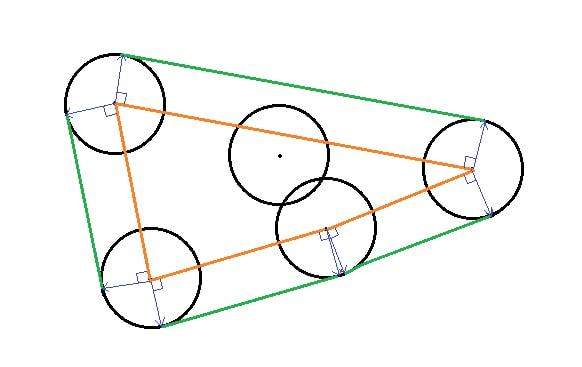
\includegraphics[scale=0.65]{Img2}
  \caption{Ilustracja algorytmu}
  \label{fig:img2}
  \end{center}
\end{figure}

Mamy efektywne algorytmy do obliczania otoczki wypukłęj dla $n$ punktów. Jednym
z nich jest algorytm Grahama, którego złożoność obliczeniowa jest $O(n\log n)$.
Ponieważ rozszerzenie otoczki wypukłej $S'$ do $S$ ma złożoność $O(n)$, to cały algorytm jest $O(n\log n)$.

\end{document}
